% !TeX root = ../Book1.tex
\begin{figure}[htbp]
	\centering
	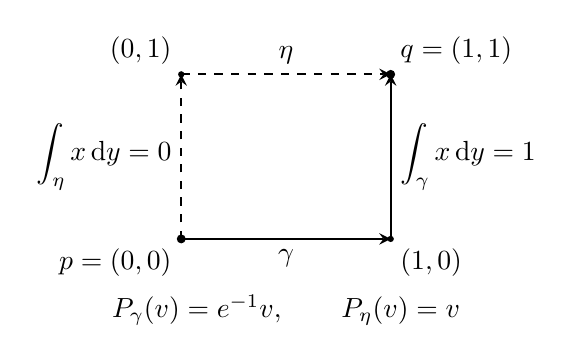
\begin{tikzpicture}[>=stealth,scale=0.95]
		\draw[thick,->] (0,0)--(2.8,0) node[midway,below] {\(\gamma\)};
		\draw[thick,->] (2.8,0)--(2.8,2.2);
		\draw[dashed,thick,->] (0,0)--(0,2.2);
		\draw[dashed,thick,->] (0,2.2)--(2.8,2.2) node[midway,above] {\(\eta\)};
		\fill (0,0) circle (1.7pt) node[below left] {\(p=(0,0)\)};
		\fill (2.8,2.2) circle (1.7pt) node[above right] {\(q=(1,1)\)};
		\fill (2.8,0) circle (1.2pt) node[below right] {\((1,0)\)};
		\fill (0,2.2) circle (1.2pt) node[above left] {\((0,1)\)};
		\node[left] at (0,1.1) {\(\displaystyle\int_\eta x\,\mathrm{d}y=0\)};
		\node[right] at (2.8,1.1) {\(\displaystyle\int_\gamma x\,\mathrm{d}y=1\)};
		\node at (1.4,-0.95) {\(P_\gamma(v)=e^{-1}v,\qquad P_\eta(v)=v\)};
	\end{tikzpicture}
	\caption{同一个联络 \(\alpha=x\,\mathrm{d}y\) 沿两条路径比较相同的两个纤维，得到不同线性同构。实线路径先水平后竖直，虚线路径的顺序相反。}
	\label{g1:fig:path-transport}
\end{figure}
